\hspace{0.5cm} This paper employs a dataset of Spanish business news articles sourced from Dow Jones Newswires, covering the period from June 24, 2020, to September 30, 2021. The selection of this timeframe is deliberate, driven by two key considerations. First, we aim to test a novel methodology on a relatively small dataset to ensure feasibility and demonstrate its utility in understanding market reactions to news. Our goal is not to conduct a big data analysis, but rather to showcase the methodology's potential on a manageable dataset. Second, to evaluate the extrapolative power of the proposed methodology, it is important that the data span a period characterized by instability and volatility, which is why we focus on the Covid-19 era.

The dataset consists of high-quality articles that have been filtered to include only those mentioning Spanish publicly traded firms listed on the IBEX-35 index. These 35 companies represent the largest firms in Spain by market capitalization and are typically the most liquid and actively traded Spanish stocks. Moreover, these companies tend to receive the most consistent media coverage, making them ideal for the scope of our analysis.

The use of Dow Jones Newswires as our news source is also intentional. Dow Jones has a standard practice of including the stock market ticker of firms directly affected by the article in parentheses, which significantly facilitates the extraction of named entities (i.e., Named Entity Recognition, or NER). The tickers used by Dow Jones align with those employed by Yahoo Finance, enabling seamless integration between our NER algorithm and subsequent firm-specific trading operations via the Yahoo Finance API.

Specifically, we employ a pattern recognition algorithm (using the \texttt{regex} library in Python) to identify firm-specific mentions of IBEX-35 companies by searching for patterns of the form \qquote{(<WORD>.MC)} for any \qquote{<WORD>}. For instance, consider the following example article (translated into English for convenience):

\begin{news}
    [A news article about Telef�nica and Cellnex]    % Caption
    [news:cellnex-article]                            % Reference
    {Cellnex will face more competition in Europe} Telef�nica's \red{(TEF.MC)} subsidiary, Telxius Telecom, has agreed to sell its telecommunications tower division in Europe and Latin America to American Tower (AMT), which will expand the latter's presence in Europe and increase competition for the Spanish wireless telecommunications group Cellnex Telecom \red{(CLNX.MC)}, according to Equita Sim. The transaction "represents the entry of a new independent tower operator into the Spanish market and potentially more competition for future growth in the European market as well," says the brokerage firm.
\end{news}

Our NER algorithm successfully identifies \texttt{TEF.MC} (Telef�nica) and \texttt{CLNX.MC} (Cellnex Telecom) as the entities directly impacted by the news article. To enhance the reliability of firm identification, we further validate the extracted entities using a Large Language Model (LLM).
In particular, we feed the articles to the LLM, which parses them according to a predefined schema. The first task in this schema is to identify all the Spanish firms listed on the IBEX-35 that are directly affected by the shocks described in the news article. 
Due to the high quality of the dataset, the correlation between entities identified by the LLM and those extracted via pattern recognition is almost exact.

For subsequent analysis, we partition the dataset into three splits: \textit{Train}, \textit{Validation}, and \textit{Test}. Each split serves a distinct purpose that will be explained in detail as we progress through the paper. Summary statistics for each data split are provided in \cref{tab:Articles_Summary_Statistics}.

%----------------------------------------------------
\inserthere{tab:Articles_Summary_Statistics}

\begin{table}[H]
\centering
\caption{Summary Statistics of Articles by Data Split}
\label{tab:Articles_Summary_Statistics}
%\begin{tabular}{|l||c|c|c|c|}
\begin{tabular}{lcccc}
\hline \Xhline{2\arrayrulewidth}
%\rowcolor{gray!10}
\textbf{Data Split} & \textbf{Time Period} & \textbf{\# Articles} & \textbf{\# Words} & \textbf{Vocabulary Size} \\
\hline \Xhline{2\arrayrulewidth}
Train & 24/06/2020 $-$ 12/02/2021 & 1254 & 327413 & 26762 \\
Validation & 12/02/2021 $-$ 21/06/2021 & 836 & 232912 & 22265 \\
Test & 21/06/2021 $-$ 30/09/2021 & 523 & 140495 & 16474 \\ \hline \Xhline{\arrayrulewidth}
All & 24/06/2020 $-$ 30/09/2021 & 2613 & 700820 & 42603 \\ \hline \Xhline{2\arrayrulewidth}
\end{tabular}
\mx 
\subcaption*{\textit{Note: Summary statistics by data splits and for the whole sample. We provide the period spanned by each data split, the number of articles, the number of words, and the vocabulary size. Articles have been preprocessed following standard NLP practices.}}
\end{table}

%----------------------------------------------------

The most frequently used words in the entire dataset are depicted in \cref{fig:WordCloud} by means of a WordCloud. As shown, the most prominent words include \qquote{empresa} (firm), \qquote{compa��a} (company), and \qquote{espa�a} (Spain), reinforcing that the dataset primarily comprises Spanish business news, with a prevalence of technical terms such as \qquote{beneficio neto} (net profit), \qquote{precio objetivo} (target price), \qquote{proyecto} (project), and \qquote{operaci�n} (operation).

%----------------------------------------------------
\inserthere{fig:WordCloud}
\begin{figure}[H]
  \centering
  \caption{Word Cloud of the Entire Dataset}
  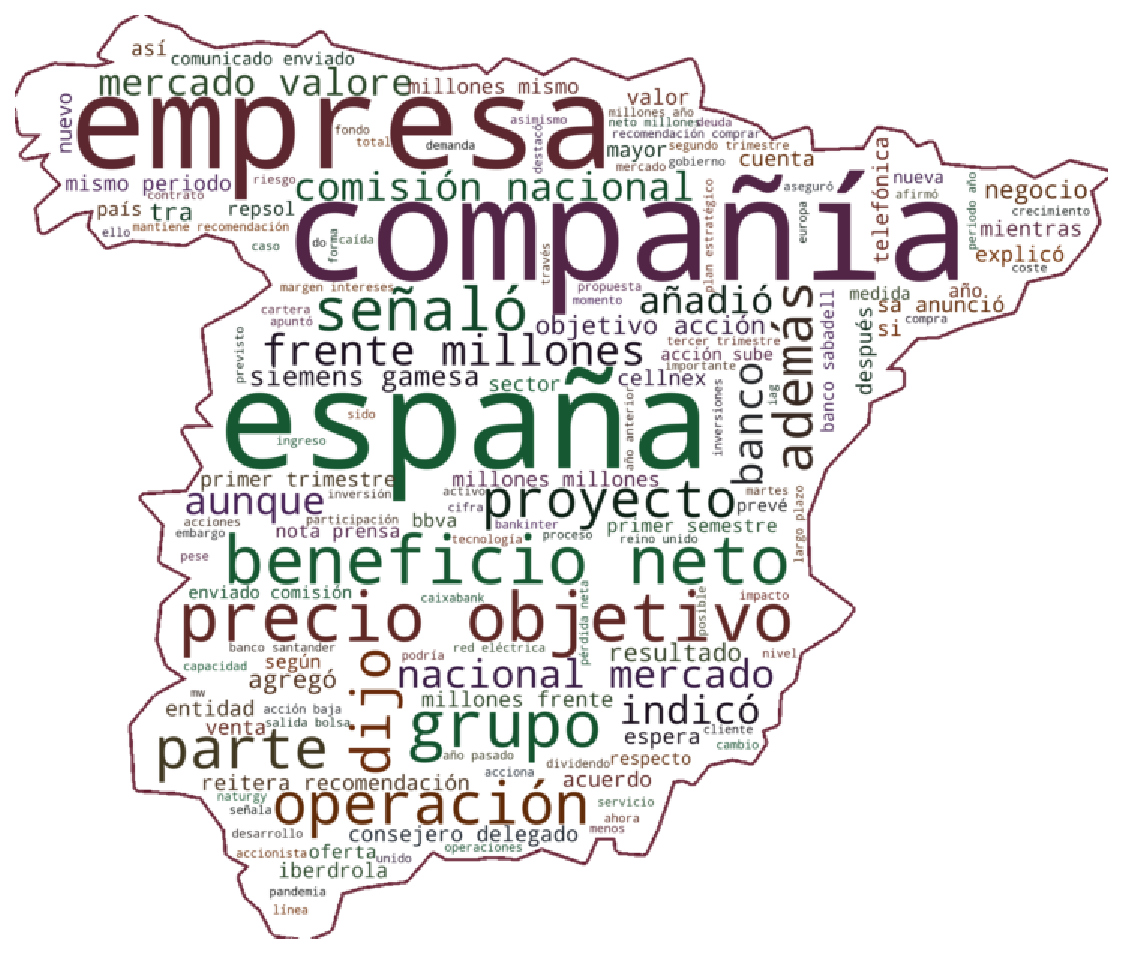
\includegraphics[scale=0.496]{/Users/jesusvillotamiranda/Library/CloudStorage/OneDrive-UniversidaddeLaRioja/CEMFI/__MSc__/__Second_year__/6th_Term/MasterThesis/__Output/EDA_WordCloud.pdf}
  \label{fig:WordCloud}
\end{figure}
%----------------------------------------------------

The distribution of the number of articles published per day is illustrated in \cref{fig:hist_1}, showing that the most frequent publication rate is between 5 and 10 articles per day, though some days exhibit unusually high publication counts. \cref{fig:hist_2} shows the distribution of the number of words per article, with the majority of articles containing between 70 and 280 words. This indicates that the articles are relatively succinct, providing direct information. However, a small subset of articles exceeds 500 words, indicating more in-depth coverage.

%----------------------------------------------------
\inserthere{fig:histograms}
\begin{figure}[H]
  \caption{Histogram of \# News Articles per Day and \# Words per Article}
  \centering
  \begin{subfigure}[b]{0.46\textwidth}
    \centering
    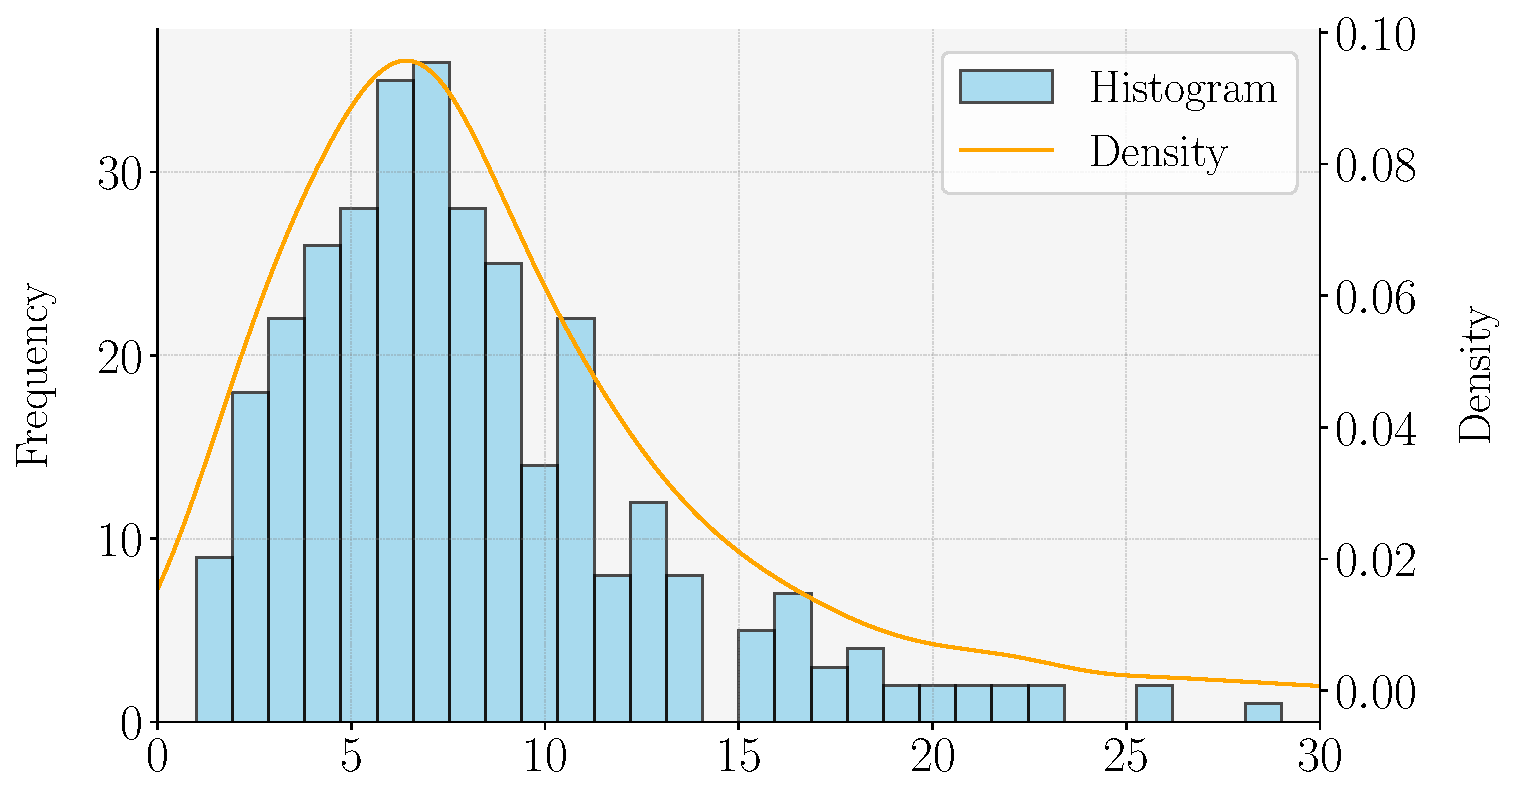
\includegraphics[width=\textwidth]{/Users/jesusvillotamiranda/Library/CloudStorage/OneDrive-UniversidaddeLaRioja/CEMFI/__MSc__/__Second_year__/6th_Term/MasterThesis/__Output/EDA_Histogram_of_Number_of_News_Articles_per_day.pdf}
    \caption{Number of News Articles per Day}
    \label{fig:hist_1}
  \end{subfigure}
  \hspace{0.05\textwidth} % Add horizontal space between the subfigures
  \begin{subfigure}[b]{0.46\textwidth}
    \centering
    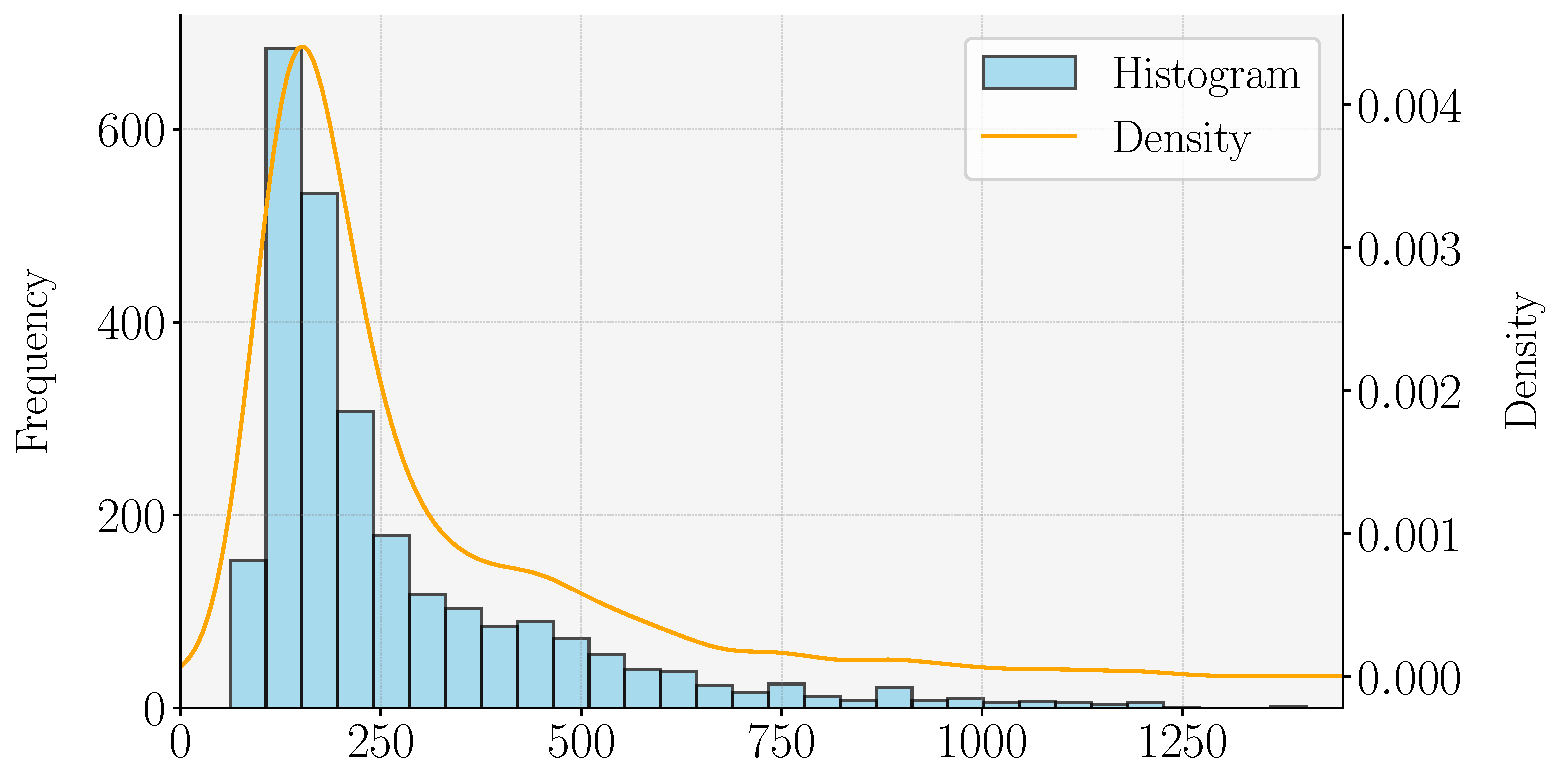
\includegraphics[width=\textwidth]{/Users/jesusvillotamiranda/Library/CloudStorage/OneDrive-UniversidaddeLaRioja/CEMFI/__MSc__/__Second_year__/6th_Term/MasterThesis/__Output/EDA_Number_of_Words_per_Article.pdf}
    \caption{Number of Words per Article}
    \label{fig:hist_2}
  \end{subfigure}
  \label{fig:histograms}
\end{figure}
%----------------------------------------------------

The time series of the number of articles published per day throughout the sample period is shown in \Cref{fig:ts_articles}. The series exhibits considerable variability, with frequent fluctuations from fewer than 5 articles per day to sudden spikes exceeding 20 articles. The 30-day moving average smooths the series, confirming the previous observation that, on average, between 5 and 10 articles are published daily.

%----------------------------------------------------
\inserthere{fig:ts_articles}
\begin{figure}[H]
  \centering
  \caption{Time Series of Number of Articles per Day and 30-Period Moving Average}
  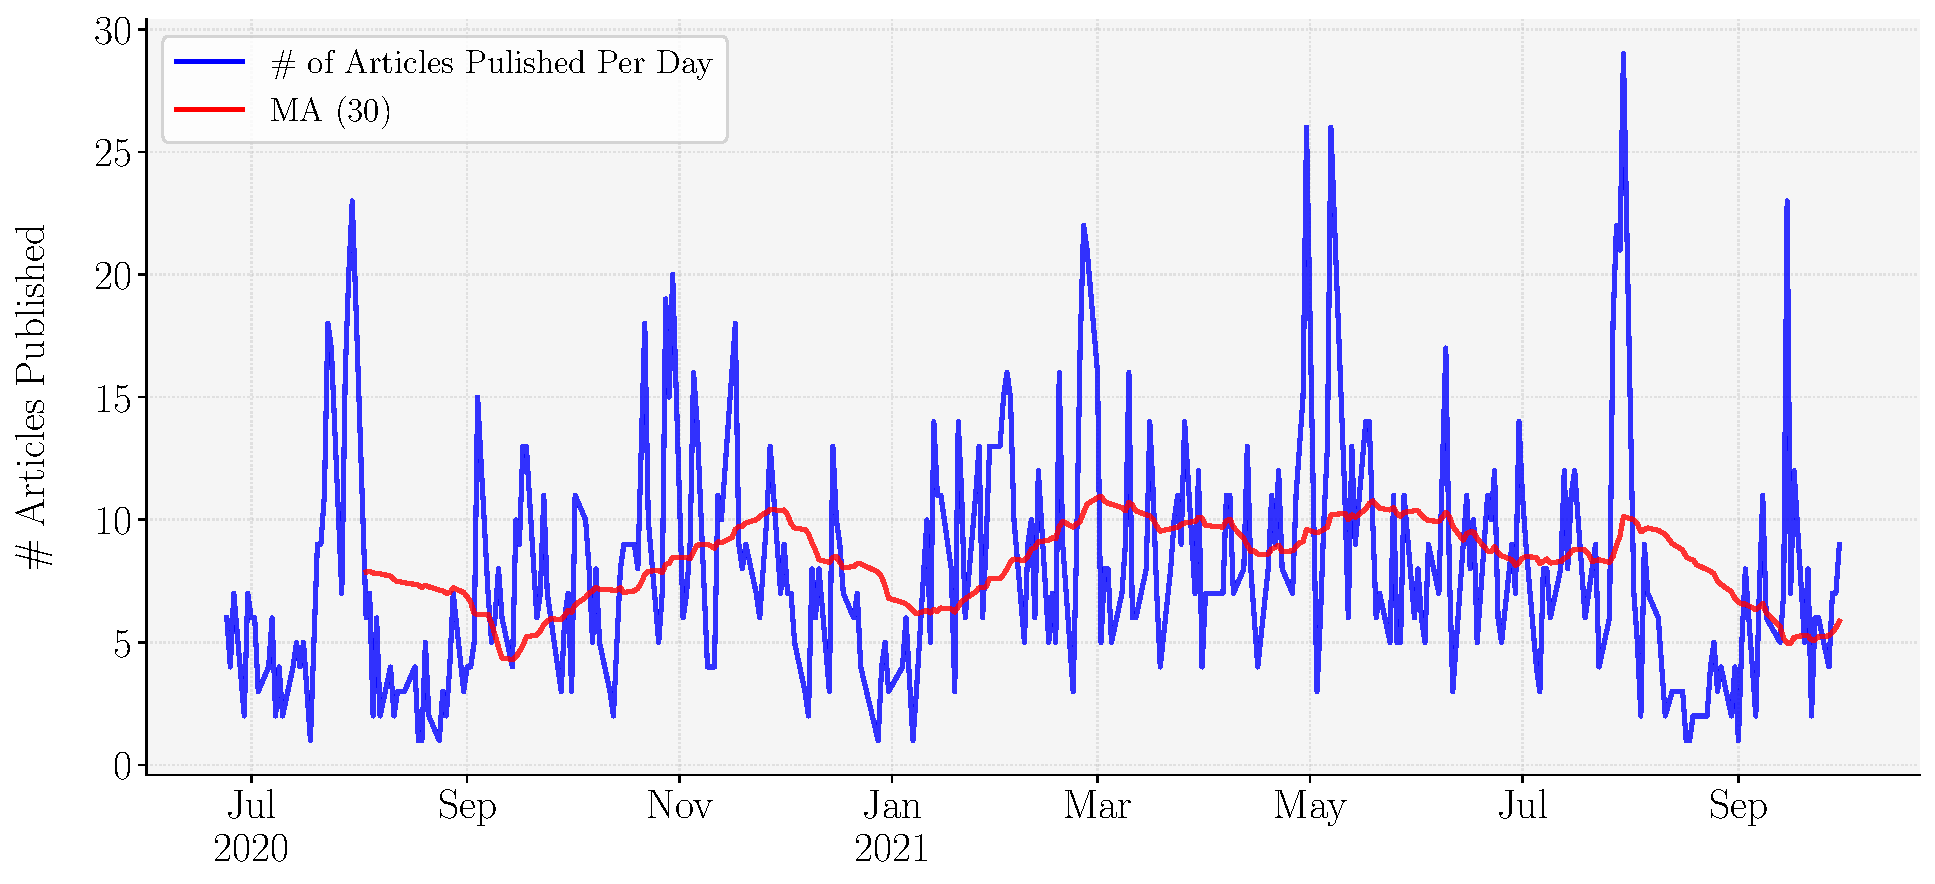
\includegraphics[scale=0.445]{/Users/jesusvillotamiranda/Library/CloudStorage/OneDrive-UniversidaddeLaRioja/CEMFI/__MSc__/__Second_year__/6th_Term/MasterThesis/__Output/EDA_Time_Series_of_Articles.pdf}
  \label{fig:ts_articles}
\end{figure}
%----------------------------------------------------